% ------------------------------------------------------------------------
\chapter{Heuristic Models}

Heuristic algorithms are used in this report with an objective to minimize the total CAPEX of the network. It is important to have these comparison results with the linear programming ones, because these formulations are faster than the optimal methods and can generate also a near optimal solution. Another advantage of the heuristic approach is that heuristic solutions leads to good performances in practical network scenarios when we present a sufficiently feasible solution, instead of an optimal solution.

In order to get the total network cost for the reference network, the CAPEX is calculated by routing and grooming heuristic algorithms implemented in Java and it is considered that all network equipment is bidirectional. These algorithms are tested in a network design software called Net2Plan.

This chapter consists in demonstrating how the matrices are created, how the heuristic algorithms work and analyzing the results. It is divided in six subsections and the results differ into three different transport modes: opaque (link-by-link grooming method), transparent (single-hop grooming method) and translucent (multi-hop grooming method). Each one of these transport methods are also distinguished and compared by the possibility of being without survivability or with 1+1 protection and for the cases of low, medium and high traffic in the network.

%Section CAPEX
\clearpage

\section{CAPEX}
\begin{tcolorbox}	
\begin{tabular}{p{2.75cm} p{0.2cm} p{10.5cm}} 	
\textbf{Student Name}  &:& Pedro Coelho    (March 01, 2018 - )\\
\textbf{Goal}          &:& Implement of the heuristic model to obtain the best possible CAPEX of a given network.
\end{tabular}
\end{tcolorbox}
\vspace{11pt}

The total CAPEX of a network, as it was already described in \ref{Capex}, is the sum between two differentiated costs. Firstly, the link cost depends on the link length, which has integrated components such as OLTs, transceivers and amplifiers and the node cost depends on the traffic intensity by each node. The optical node cost is 0 because all the ports in the network are electrical.

In order to get the results for the heuristic approach, routing and grooming algorithms are used which try to obtain the most near optimal solution for the six cases detailed in this chapter. Then, it will be applied a cost report with all the detailed information about the costs of the network. The final CAPEX depends on the transport mode (opaque, transparent and translucent), possibility of the network having a dedicated 1+1 protection scheme or not and the network traffic (low - 0.5 Tbit/s, medium - 5 Tbit/s and high - 10 Tbit/s).

To calculate the total network cost it has to be considered the links cost and the nodes cost. The CAPEX value of a network is calculated by the equation \ref{Capex_heuristic}.

\begin{equation}
C_C = C_L + C_N
\label{Capex_heuristic}
\end{equation}

\begin{itemize}
\item Where {$C_L$ is the link cost in monetary units (e.g. euros, or dollars)}.
\item Where {$C_N$ is the node cost in monetary units (e.g. euros, or dollars)}.
\end{itemize}

On the first hand, the link cost, in monetary units (e.g. euros, or dollars), is calculated by the equation \ref{Capex_Link_heuristic}. If the length of the link is longer, the resulting costs will be higher due to of the necessity of having more components which carry all the traffic from all origin nodes to all destination nodes.

\begin{equation}
C_L = \sum_{i=1}^N \sum_{j=i+1}^N L_{ij} \left( 2 \gamma_0^{OLT} + 2 \gamma_1^{OLT} \tau W_{ij} + N^R_{ij} c^R \right)
\label{Capex_Link_heuristic}
\end{equation}

\begin{itemize}
\item Where {$i$ is the index for start node of a physical link}.
\item Where {$j$ is the index for end node of a physical link}.
\item Where {$N$ is the total number of nodes, N $\in \mathbb{N}$}.
\item Where {$L_{ij}$ is the binary variable indicating if link between the nodes $i$ and $j$ is used, $L_{ij} \in {0, 1}$}.
\item Where {$\gamma_0^{OLT}$ is the OLT cost in monetary units (e.g. euros, or dollars)}.
\item Where {$\gamma_1^{OLT}$ is the transponder cost in monetary units (e.g. euros, or dollars)}.
\item Where {$\tau$ is the line bit-rate}.
\item Where {$W_{ij}$ is the number of optical channels in link $i$ $j$}.
\item Where {$N^R_{ij}$ is the number of optical amplifiers in link $i$ $j$}.
\item Where {$c^R$ is the optical amplifiers cost in monetary units (e.g. euros, or dollars)}.
\end{itemize}

The line bit-rate that is used in this report has the value of 100. It represents the separation between regeneration stages in km.

On the other hand, the nodes cost, in monetary units (e.g. euros, or dollars), is calculated by the equation \ref{Capex_Node_heuristic}.

\begin{equation}
C_N = C_{EXC} + C_{OXC}
\label{Capex_Node_heuristic}
\end{equation}

\begin{itemize}
\item Where {$C_{EXC}$ is the electrical node cost in monetary units (e.g. euros, or dollars)}.
\item Where {$C_{OXC}$ is the optical node cost in monetary units (e.g. euros, or dollars)}.
\end{itemize}

\vspace{11pt}
As all the nodes have an electrical part and an optical part, so it is necessary to calculate both with their respective formulas and sum the results.

The electrical node cost, in monetary units (e.g. euros, or dollars), is given by the equation \ref{Capex_Node_EXC_heuristic}.

\begin{equation}
C_{EXC} = \sum_{n=1}^{N} N_{exc,n} \left( \gamma_{e0} + \sum_{c=-1}^B \gamma_{e1,c} P_{exc,c,n} \right)
\label{Capex_Node_EXC_heuristic}
\end{equation}

\begin{itemize}
\item Where {$N$ is the total number of nodes, N $\in \mathbb{N}$}.
\item Where {$N_{exc,n}$ is the binary variable indicating if node $n$ is used, $N_{exc,n} \in {0, 1}$}.
\item Where {$\gamma_{e0}$ is the EXC cost in monetary units (e.g. euros, or dollars)}.
\item Where {$\gamma_{e1,c}$ is the EXC port cost in monetary units (e.g. euros, or dollars) with bit-rate $B$ and with a given transceiver reach}.
\item Where {$P_{exc,c,n}$ is the number of ports of the electrical switch}.
\item Where {$B$ is a natural number corresponding to the maximum index of short-reach ports, see table below}.
\end{itemize}

\begin{table}[H]
\centering
\begin{tabular}{|c|c|}
  \hline
  Index & Bit rate \\
 \hline\hline
  -1 & 100 Gbits/s line bit-rate (long-reach port) \\
  0 & 1.25 Gbits/s tributary bit-rate (short-reach port) \\
  1 & 2.5 Gbits/s tributary bit-rate (short-reach port) \\
  2 & 10 Gbits/s tributary bit-rate (short-reach port) \\
  3 & 40 Gbits/s tributary bit-rate (short-reach port) \\
  4 & 100 Gbits/s tributary bit-rate (short-reach port) \\
  \hline
\end{tabular}
\caption{Table with index and your corresponding bit rate}
\label{table_bitrate}
\end{table}

The constitution of the electrical node part can be seen in the Integer Linear Programming section \ref{exc_design}.

Finally, the optical cost, in monetary units (e.g. euros, or dollars), is given by equation \ref{Capex_Node_OXC_heuristic}.

\begin{equation}
C_{OXC} = \sum_{n=1}^{N} N_{oxc,n} \left( \gamma_{o0} + \gamma_{o1} P_{oxc,n} \right)
\label{Capex_Node_OXC_heuristic}
\end{equation}

\begin{itemize}
\item Where {$N$ is the total number of nodes, N $\in \mathbb{N}$}.
\item Where {$N_{oxc,n}$ is the binary variable indicating if node $n$ is used, $N_{oxc,n} \in {0, 1}$}.
\item Where {$\gamma_{o0}$ is the OXC cost in monetary units (e.g. euros, or dollars)}.
\item Where {$\gamma_{o1}$ is the OXC port cost in monetary units (e.g. euros, or dollars) }.
\item Where {$P_{oxc,n}$ is the number of ports of the optical switch}.
\end{itemize}

The constitution of the optical node part can be seen in the Integer Linear Programming section \ref{oxc_design}.

After all the formulas needed to calculate the CAPEX of a network are demonstrated above, it is also essential to have pre-defined the costs of the network equipments. In the table \ref{table_cost_heuristic} it is shown the cost, in euros, of all the equipments with their symbols used in the respective formulas.\\

\begin{table}[H]
\centering
\begin{tabular}{|| c | c | c||}
 \hline
 Equipment & Symbol & Cost \\
 \hline\hline
 OLT without transponders & $\gamma_0^{OLT}$ & 15000 \euro \\
 Transponder & $\gamma_1^{OLT}$ & 5000 \euro/Gb \\
 Unidirectional Optical Amplifier & $c^R$ & 4000 \euro \\
 EXC & $\gamma_{e0}$ & 10000 \euro \\
 OXC & $\gamma_{o0}$ & 20000 \euro \\
 EXC Port for line ports & $\gamma_{e1,-1}$ & 1000 \euro /Gb/s\\
 EXC Port for ODU0 & $\gamma_{e1,0}$ & 8 \euro /Gb/s\\
 EXC Port for ODU1 & $\gamma_{e1,1}$ & 6 \euro /Gb/s\\
 EXC Port for ODU2 & $\gamma_{e1,2}$ & 3 \euro /Gb/s\\
 EXC Port for ODU3 & $\gamma_{e1,3}$ & 1.5 \euro /Gb/s\\
 EXC Port for ODU4 & $\gamma_{e1,4}$ & 1 \euro /Gb/s\\
 OXC Port & $\gamma_{o1}$ & 2500 \euro /porto \\
 \hline
\end{tabular}
\caption{Table with costs}
\label{table_cost_heuristic}
\end{table}

%Subsection with the different transport mode
\clearpage

\subsection{Opaque without Survivability}\label{heuristic_Opaque_Survivability}
\begin{tcolorbox}	
\begin{tabular}{p{2.75cm} p{0.2cm} p{10.5cm}} 	
\textbf{Student Name}  &:& Pedro Coelho    (March 01, 2018 - )\\
\textbf{Goal}          &:& Implement the Heuristic model for the opaque transport mode without survivability.
\end{tabular}
\end{tcolorbox}

\subsubsection{Model description}
\vspace{11pt}
In the opaque transport mode (link-by-link approach), the lightpath entering any intermediate node is necessarily terminated, i.e., there are performed OEO (optical-electrical-optical) conversions at every intermediate node since the origin to the destination node. These conversions are used for every wavelength at every node.

Contrary to the opaque with dedicated 1+1 protection technique, the opaque without survivability technique does not have a backup path, so if there is a network failure it is more likely to suffer large data losses, which consequently leads to higher network costs. However, the CAPEX will be significantly lower, because that not includes a secondary path that would increase several network elements.

For this model, after the creation of the matrices and the network topology, it is necessary to apply the routing and grooming algorithms created. For the "Logical Topology" algorithm, the user must insert "Opaque" in the "logicalTopology" value and for the "Grooming" algorithm, the user must insert "no" in the parameter value "protection".

At the end, the "Cost Report" algorithm will be applied to obtain the best CAPEX result for the network in question.

Firstly, in the opaque transport mode, the optical node cost is 0 because all the ports in the network are electrical. Consequently, to calculate the node cost it only has to be considered the electrical node cost.

\begin{itemize}
  \item Where $N_{OXC,n}$ = 0, \quad $\forall$ n.
  \item Where $N_{EXC,n}$ = 1, \quad $\forall$ n that process traffic.
\end{itemize}

Still referring to the electrical node cost, the number of long-reach ports of the electrical switch, i.e., the number of line ports of a node n is calculated by the equation \ref{EXC_pexc1_opaque_heuristic}.

\begin{equation}
P_{exc,-1,n} = \sum_{j=1}^{N} w_{nj}
\label{EXC_pexc1_opaque_heuristic}
\end{equation}

\begin{itemize}
\item Where {$w_{nj}$ is the number of optical channels between node $n$ and node $j$}.
\end{itemize}

\newpage
\vspace{11pt}
In addition, the number of short-reach ports of the electrical switch, i.e., the number of tributary ports with bit-rate c in a node n is calculated by the equation \ref{EXC_pexc2_opaque_heuristic}.

\begin{equation}
P_{exc,c,n} = \sum_{d=1}^{N} D_{nd,c}
\label{EXC_pexc2_opaque_heuristic}
\end{equation}

\begin{itemize}
  \item Where {$D_{nd,c}$ are the client demands between nodes $n$ and $d$ with bit rate $c$}.
\end{itemize}

\vspace{11pt}
In this case there is the following particularity:

\begin{itemize}
  \item When $n$=$j$, the value of client demands is always zero, i.e, $D_{nn,c}=0$.
\end{itemize}

\subsubsection{Result description}

It is already known all the necessary formulas to obtain the CAPEX value for the reference network \ref{Reference_Network_Topology}. As described in the subsection of the network traffic \ref{Reference_Network_Traffic}, it is necessary to obtain three different values of CAPEX for the low (0.5 Tbit/s), medium (5 Tbit/s) and high (10 Tbit/s) traffic. It is used a network software program called Net2Plan which can design the traffic matrices, create all the network topologies, simulate the algorithms into the network implemented in the programming software called Eclipse and analyze the results obtained.\\

\textbf{Low Traffic Scenario:}\\

In this scenario it has to take into account the traffic calculated in \ref{low_traffic_scenario}. In a first phase it will be shown the three topologies of the network, the first one already knew allowed physical topology, the second one allowed optical topology and finally the physical topology.\\

\textbf{0.5 Tbit/s}

\begin{figure}[H]
\centering
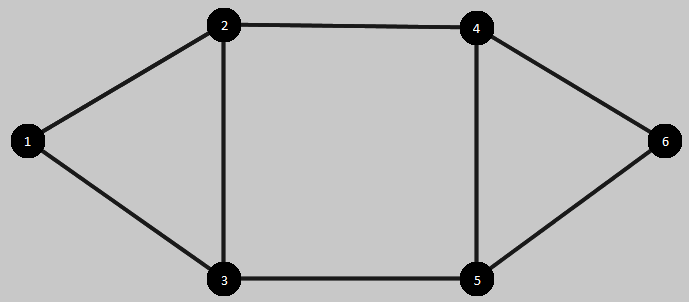
\includegraphics[width=13cm]{sdf/heuristic/figures/topological_design1}
\caption{Allowed physical topology of the reference network.}
\label{allowed_physical_surv_ref_low_heuristic}
\end{figure}

Following all the steps mentioned in the \ref{net2plan_guide}, applying the routing and grooming heuristic algorithms in the Net2Plan software and using all the data referring to this scenario, the obtained result can be consulted in the following table:

\begin{table}[H]
\centering
\begin{tabular}{|| c | c | c | c | c | c | c ||}
 \hline
 \multicolumn{7}{|| c ||}{CAPEX of the Network} \\
 \hline
 \hline
 \multicolumn{3}{|| c |}{ } & Quantity & Unit Price & Cost & Total \\
 \hline
 \multirow{3}{*}{Link Cost} & \multicolumn{2}{ c |}{OLTs} & 16 & 15 000 \euro & 240 000 \euro & \multirow{3}{*}{13 520 000 \euro} \\ \cline{2-6}
 & \multicolumn{2}{ c |}{100 Gb/s Transceivers} & 26 & 5 000 \euro/Gb/s & 13 000 000 \euro & \\ \cline{2-6}
 & \multicolumn{2}{ c |}{Amplifiers} & 70 & 4 000 \euro & 280 000 \euro & \\
 \hline
 \multirow{9}{*}{Node Cost} & \multirow{7}{*}{Electrical} & EXCs & 6 & 10 000 \euro & 60 000 \euro & \multirow{9}{*}{2 662 590 \euro} \\ \cline{3-6}
 & & ODU0 Ports & 60 & 8 \euro/Gb/s & 600 \euro & \\ \cline{3-6}
 & & ODU1 Ports & 50 & 6 \euro/Gb/s & 750 \euro & \\ \cline{3-6}
 & & ODU2 Ports & 16 & 3 \euro/Gb/s & 480 \euro & \\ \cline{3-6}
 & & ODU3 Ports & 6 & 1.5 \euro/Gb/s & 360 \euro & \\ \cline{3-6}
 & & ODU4 Ports & 4 & 1 \euro/Gb/s & 400 \euro & \\ \cline{3-6}
 & & Line Ports & 26 & 1 000 \euro/Gb/s & 2 600 000 \euro & \\ \cline{2-6}
 & \multirow{2}{*}{Optical} & OXCs & 0 & 20 000 \euro & 0 \euro & \\ \cline{3-6}
 & & Ports & 0 & 2 500 \euro/porto & 0 \euro & \\
 \hline
 \multicolumn{6}{|| c |}{Total Network Cost} & 16 182 590 \euro \\
\hline
\end{tabular}
\caption{Table with detailed description of CAPEX}
\label{scriptopaque_surv_ref_low_heuristic}
\end{table}

Through the formulas mentioned below it can be demonstrated how all the values of the quantity column were calculated.

\begin{equation*}
 OLTs: 2 \sum_{(i,j):i<j}L_{ij} \qquad \qquad
 Transceivers: 2 \sum_{(i,j):i<j}W_{ij} \qquad \qquad
 Amplifiers: \sum_{(i,j):i<j}N^R_{ij} L_{ij} \\
\end{equation*}
\begin{equation*}
 EXCs: \sum_n^N N_{EXC,n} \qquad
 ODU0: \sum_{(o,d)}^{N}D_{od,0} \qquad \qquad
 ODU1: \sum_{(o,d)}^{N}D_{od,1} \qquad
 ODU2: \sum_{(o,d)}^{N}D_{od,2}
\end{equation*}
\begin{equation*}
 ODU3: \sum_{(o,d)}^{N}D_{od,3} \qquad \qquad
 ODU4: \sum_{(o,d)}^{N}D_{od,4} \qquad \qquad
 Line: \sum_{(i,j)}^{N}W_{ij}
\end{equation*}

\vspace{13pt}
$OXCs: \sum_n^N N_{OXC,n}$ but as mentioned initially this result is always zero \\

$Ports$: does not exist for this case then it is equal to zero \\

\newpage
\textbf{Medium Traffic Scenario:}\\

In this scenario it has to take into account the traffic calculated in \ref{medium_traffic_scenario}. In a first phase it will be shown the three topologies of the network, the first one already knew allowed physical topology, the second one allowed optical topology and finally the physical topology.\\

\textbf{5 Tbit/s}

\begin{figure}[H]
\centering
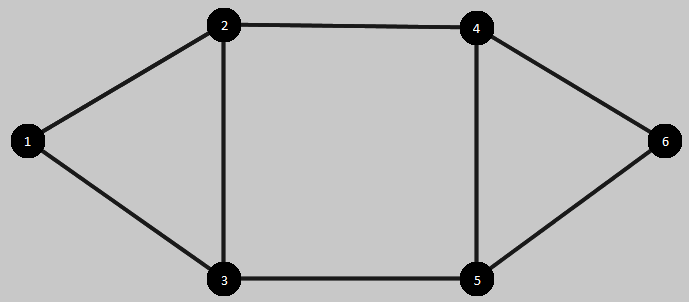
\includegraphics[width=13cm]{sdf/heuristic/figures/topological_design1}
\caption{Allowed physical topology of the reference network.}
\label{allowed_physical_surv_ref_low_heuristic}
\end{figure}

Following all the steps mentioned in the \ref{net2plan_guide}, applying the routing and grooming heuristic algorithms in the Net2Plan software and using all the data referring to this scenario, the obtained result can be consulted in the following table:

\begin{table}[H]
\centering
\begin{tabular}{|| c | c | c | c | c | c | c ||}
 \hline
 \multicolumn{7}{|| c ||}{CAPEX of the Network} \\
 \hline
 \hline
 \multicolumn{3}{|| c |}{ } & Quantity & Unit Price & Cost & Total \\
 \hline
 \multirow{3}{*}{Link Cost} & \multicolumn{2}{ c |}{OLTs} & 16 & 15 000 \euro & 240 000 \euro & \multirow{3}{*}{94 520 000 \euro} \\ \cline{2-6}
 & \multicolumn{2}{ c |}{100 Gb/s Transceivers} & 188 & 5 000 \euro/Gb/s & 94 000 000 \euro & \\ \cline{2-6}
 & \multicolumn{2}{ c |}{Amplifiers} & 70 & 4 000 \euro & 280 000 \euro & \\
 \hline
 \multirow{9}{*}{Node Cost} & \multirow{7}{*}{Electrical} & EXCs & 6 & 10 000 \euro & 60 000 \euro & \multirow{9}{*}{18 862 590 \euro} \\ \cline{3-6}
 & & ODU0 Ports & 60 & 8 \euro/Gb/s & 600 \euro & \\ \cline{3-6}
 & & ODU1 Ports & 50 & 6 \euro/Gb/s & 750 \euro & \\ \cline{3-6}
 & & ODU2 Ports & 16 & 3 \euro/Gb/s & 480 \euro & \\ \cline{3-6}
 & & ODU3 Ports & 6 & 1.5 \euro/Gb/s & 360 \euro & \\ \cline{3-6}
 & & ODU4 Ports & 4 & 1 \euro/Gb/s & 400 \euro & \\ \cline{3-6}
 & & Line Ports & 26 & 1 000 \euro/Gb/s & 2 600 000 \euro & \\ \cline{2-6}
 & \multirow{2}{*}{Optical} & OXCs & 0 & 20 000 \euro & 0 \euro & \\ \cline{3-6}
 & & Ports & 0 & 2 500 \euro/porto & 0 \euro & \\
 \hline
 \multicolumn{6}{|| c |}{Total Network Cost} & 113 382 590 \euro \\
\hline
\end{tabular}
\caption{Table with detailed description of CAPEX}
\label{scriptopaque_surv_ref_medium_heuristic}
\end{table}

Through the formulas mentioned below it can be demonstrated how all the values of the quantity column were calculated.

\begin{equation*}
 OLTs: 2 \sum_{(i,j):i<j}L_{ij} \qquad \qquad
 Transceivers: 2 \sum_{(i,j):i<j}W_{ij} \qquad \qquad
 Amplifiers: \sum_{(i,j):i<j}N^R_{ij} L_{ij} \\
\end{equation*}
\begin{equation*}
 EXCs: \sum_n^N N_{EXC,n} \qquad
 ODU0: \sum_{(o,d)}^{N}D_{od,0} \qquad \qquad
 ODU1: \sum_{(o,d)}^{N}D_{od,1} \qquad
 ODU2: \sum_{(o,d)}^{N}D_{od,2}
\end{equation*}
\begin{equation*}
 ODU3: \sum_{(o,d)}^{N}D_{od,3} \qquad \qquad
 ODU4: \sum_{(o,d)}^{N}D_{od,4} \qquad \qquad
 Line: \sum_{(i,j)}^{N}W_{ij}
\end{equation*}

\vspace{13pt}
$OXCs: \sum_n^N N_{OXC,n}$ but as mentioned initially this result is always zero \\

$Ports$: does not exist for this case then it is equal to zero \\

\textbf{High Traffic Scenario:}\\

In this scenario it has to take into account the traffic calculated in \ref{high_traffic_scenario}. In a first phase it will be shown the three topologies of the network, the first one already knew allowed physical topology, the second one allowed optical topology and finally the physical topology.\\

\textbf{10 Tbit/s}

\begin{figure}[H]
\centering
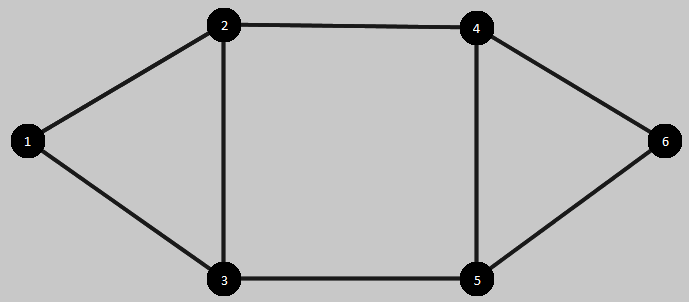
\includegraphics[width=13cm]{sdf/heuristic/figures/topological_design1}
\caption{Allowed physical topology of the reference network.}
\label{allowed_physical_surv_ref_low_heuristic}
\end{figure}

Following all the steps mentioned in the \ref{net2plan_guide}, applying the routing and grooming heuristic algorithms in the Net2Plan software and using all the data referring to this scenario, the obtained result can be consulted in the following table:

\begin{table}[H]
\centering
\begin{tabular}{|| c | c | c | c | c | c | c ||}
 \hline
 \multicolumn{7}{|| c ||}{CAPEX of the Network} \\
 \hline
 \hline
 \multicolumn{3}{|| c |}{ } & Quantity & Unit Price & Cost & Total \\
 \hline
 \multirow{3}{*}{Link Cost} & \multicolumn{2}{ c |}{OLTs} & 16 & 15 000 \euro & 240 000 \euro & \multirow{3}{*}{186 020 000 \euro} \\ \cline{2-6}
 & \multicolumn{2}{ c |}{100 Gb/s Transceivers} & 371 & 5 000 \euro/Gb/s & 185 500 000 \euro & \\ \cline{2-6}
 & \multicolumn{2}{ c |}{Amplifiers} & 70 & 4 000 \euro & 280 000 \euro & \\
 \hline
 \multirow{9}{*}{Node Cost} & \multirow{7}{*}{Electrical} & EXCs & 6 & 10 000 \euro & 60 000 \euro & \multirow{9}{*}{37 162 590 \euro} \\ \cline{3-6}
 & & ODU0 Ports & 60 & 8 \euro/Gb/s & 600 \euro & \\ \cline{3-6}
 & & ODU1 Ports & 50 & 6 \euro/Gb/s & 750 \euro & \\ \cline{3-6}
 & & ODU2 Ports & 16 & 3 \euro/Gb/s & 480 \euro & \\ \cline{3-6}
 & & ODU3 Ports & 6 & 1.5 \euro/Gb/s & 360 \euro & \\ \cline{3-6}
 & & ODU4 Ports & 4 & 1 \euro/Gb/s & 400 \euro & \\ \cline{3-6}
 & & Line Ports & 26 & 1 000 \euro/Gb/s & 2 600 000 \euro & \\ \cline{2-6}
 & \multirow{2}{*}{Optical} & OXCs & 0 & 20 000 \euro & 0 \euro & \\ \cline{3-6}
 & & Ports & 0 & 2 500 \euro/porto & 0 \euro & \\
 \hline
 \multicolumn{6}{|| c |}{Total Network Cost} & 223 182 590 \euro \\
\hline
\end{tabular}
\caption{Table with detailed description of CAPEX}
\label{scriptopaque_surv_ref_high_heuristic}
\end{table}

Through the formulas mentioned below it can be demonstrated how all the values of the quantity column were calculated.

\begin{equation*}
 OLTs: 2 \sum_{(i,j):i<j}L_{ij} \qquad \qquad
 Transceivers: 2 \sum_{(i,j):i<j}W_{ij} \qquad \qquad
 Amplifiers: \sum_{(i,j):i<j}N^R_{ij} L_{ij} \\
\end{equation*}
\begin{equation*}
 EXCs: \sum_n^N N_{EXC,n} \qquad
 ODU0: \sum_{(o,d)}^{N}D_{od,0} \qquad \qquad
 ODU1: \sum_{(o,d)}^{N}D_{od,1} \qquad
 ODU2: \sum_{(o,d)}^{N}D_{od,2}
\end{equation*}
\begin{equation*}
 ODU3: \sum_{(o,d)}^{N}D_{od,3} \qquad \qquad
 ODU4: \sum_{(o,d)}^{N}D_{od,4} \qquad \qquad
 Line: \sum_{(i,j)}^{N}W_{ij}
\end{equation*}

\vspace{13pt}
$OXCs: \sum_n^N N_{OXC,n}$ but as mentioned initially this result is always zero \\

$Ports$: does not exist for this case then it is equal to zero \\ 
\clearpage

\subsection{Opaque with 1+1 Protection}\label{heuristic_Opaque_Protection}
\begin{tcolorbox}	
\begin{tabular}{p{2.75cm} p{0.2cm} p{10.5cm}} 	
\textbf{Student Name}  &:& Pedro Coelho    (March 01, 2018 - )\\
\textbf{Goal}          &:& Implement the heuristic model for the opaque transport mode with 1 plus 1 protection.
\end{tabular}
\end{tcolorbox}

\subsubsection{Model description}

The impact of failure in WDM (Wavelength Division Multiplexing) networks is caused by extremely high volume of traffic carried. In a high speed network like the WDM, a failure of a network element may cause failure of various optical channels that leads to large data and revenue losses, which can interrupt communication services.

In this protection scheme, the primary and backup path carry the traffic end-to-end, i.e., there is a need to have a backup path (the unaffected path) in case of a network failure. Then, the receiver will decide which one of the two incoming traffic it is going to pick, if the primary or the backup path.

Although it is the fastest protection scheme, it is also the most expensive, because it normally uses more than the double of the capacity for the primary path. This happens because the backup path is typically longer than the primary.

For this protection model, after the creation of the matrices and the network topology, it is necessary to apply the routing and grooming algorithms created. For the "Logical Topology" algorithm, the user must insert "Opaque" in the "logicalTopology" value and for the "Grooming" algorithm, the user must insert "yes" in the parameter value "protection".

At the end, the "Cost Report" algorithm will be applied to obtain the best CAPEX result for the network in question.

Firstly, in the opaque transport mode, the optical node cost is 0 because all the ports in the network are electrical. Consequently, to calculate the node cost it only has to be considered the electrical node cost.

\begin{itemize}
  \item Where $N_{OXC,n}$ = 0, \quad $\forall$ n.
  \item Where $N_{EXC,n}$ = 1, \quad $\forall$ n that process traffic.
\end{itemize}

Still referring to the electrical node cost, the number of long-reach ports of the electrical switch, i.e., the number of line ports of a node n is calculated by the equation \ref{EXC_pexc1_opaque_heuristic_protec}.

\begin{equation}
P_{exc,-1,n} = \sum_{j=1}^{N} w_{nj}
\label{EXC_pexc1_opaque_heuristic_protec}
\end{equation}

\begin{itemize}
\item Where {$w_{nj}$ is the number of optical channels between node $n$ and node $j$}.
\end{itemize}

\newpage
\vspace{11pt}
In addition, the number of short-reach ports of the electrical switch, i.e., the number of tributary ports with bit-rate c in a node n is calculated by the equation \ref{EXC_pexc2_opaque_heuristic_protec}.

\begin{equation}
P_{exc,c,n} = \sum_{d=1}^{N} D_{nd,c}
\label{EXC_pexc2_opaque_heuristic_protec}
\end{equation}

\begin{itemize}
  \item Where {$D_{nd,c}$ are the client demands between nodes $n$ and $d$ with bit rate $c$}.
\end{itemize}

\vspace{11pt}
In this case there is the following particularity:

\begin{itemize}
  \item When $n$=$j$, the value of client demands is always zero, i.e, $D_{nn,c}=0$.
\end{itemize}

\subsubsection{Result description}

It is already known all the necessary formulas to obtain the CAPEX value for the reference network \ref{Reference_Network_Topology}. As described in the subsection of the network traffic \ref{Reference_Network_Traffic}, it is necessary to obtain three different values of CAPEX for the low (0.5 Tbit/s), medium (5 Tbit/s) and high (10 Tbit/s) traffic. It is used a network software program called Net2Plan which can design the traffic matrices, create all the network topologies, simulate the algorithms into the network implemented in the programming software called Eclipse and analyze the results obtained.\\

\textbf{Low Traffic Scenario:}\\

In this scenario it has to take into account the traffic calculated in \ref{low_traffic_scenario}. In a first phase it will be shown the three topologies of the network, the first one already knew allowed physical topology, the second one allowed optical topology and finally the physical topology.\\

\textbf{0.5 Tbit/s}

\begin{figure}[H]
\centering
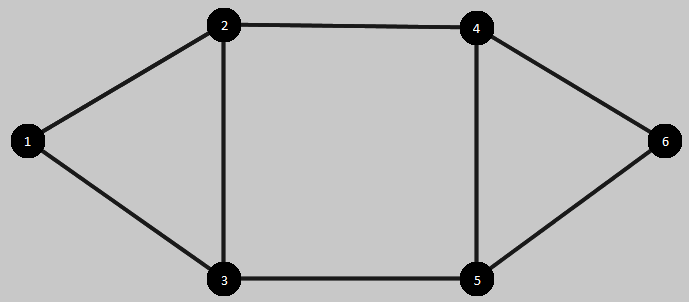
\includegraphics[width=13cm]{sdf/heuristic/figures/topological_design1}
\caption{Allowed physical topology of the reference network.}
\label{allowed_physical_surv_ref_low_heuristic}
\end{figure}

Following all the steps mentioned in the \ref{net2plan_guide}, applying the routing and grooming heuristic algorithms in the Net2Plan software and using all the data referring to this scenario, the obtained result can be consulted in the following table:

\begin{table}[H]
\centering
\begin{tabular}{|| c | c | c | c | c | c | c ||}
 \hline
 \multicolumn{7}{|| c ||}{CAPEX of the Network} \\
 \hline
 \hline
 \multicolumn{3}{|| c |}{ } & Quantity & Unit Price & Cost & Total \\
 \hline
 \multirow{3}{*}{Link Cost} & \multicolumn{2}{ c |}{OLTs} & 16 & 15 000 \euro & 240 000 \euro & \multirow{3}{*}{29 520 000 \euro} \\ \cline{2-6}
 & \multicolumn{2}{ c |}{100 Gb/s Transceivers} & 58 & 5 000 \euro/Gb/s & 29 000 000 \euro & \\ \cline{2-6}
 & \multicolumn{2}{ c |}{Amplifiers} & 70 & 4 000 \euro & 280 000 \euro & \\
 \hline
 \multirow{9}{*}{Node Cost} & \multirow{7}{*}{Electrical} & EXCs & 6 & 10 000 \euro & 60 000 \euro & \multirow{9}{*}{5 862 590 \euro} \\ \cline{3-6}
 & & ODU0 Ports & 60 & 8 \euro/Gb/s & 600 \euro & \\ \cline{3-6}
 & & ODU1 Ports & 50 & 6 \euro/Gb/s & 750 \euro & \\ \cline{3-6}
 & & ODU2 Ports & 16 & 3 \euro/Gb/s & 480 \euro & \\ \cline{3-6}
 & & ODU3 Ports & 6 & 1.5 \euro/Gb/s & 360 \euro & \\ \cline{3-6}
 & & ODU4 Ports & 4 & 1 \euro/Gb/s & 400 \euro & \\ \cline{3-6}
 & & Line Ports & 58 & 1 000 \euro/Gb/s & 5 800 000 \euro & \\ \cline{2-6}
 & \multirow{2}{*}{Optical} & OXCs & 0 & 20 000 \euro & 0 \euro & \\ \cline{3-6}
 & & Ports & 0 & 2 500 \euro/porto & 0 \euro & \\
 \hline
 \multicolumn{6}{|| c |}{Total Network Cost} & 35 382 590 \euro \\
\hline
\end{tabular}
\caption{Table with detailed description of CAPEX}
\label{scriptopaque_protec_ref_low_heuristic}
\end{table}

Through the formulas mentioned below it can be demonstrated how all the values of the quantity column were calculated.

\begin{equation*}
 OLTs: 2 \sum_{(i,j):i<j}L_{ij} \qquad \qquad
 Transceivers: 2 \sum_{(i,j):i<j}W_{ij} \qquad \qquad
 Amplifiers: \sum_{(i,j):i<j}N^R_{ij} L_{ij} \\
\end{equation*}
\begin{equation*}
 EXCs: \sum_n^N N_{EXC,n} \qquad
 ODU0: \sum_{(o,d)}^{N}D_{od,0} \qquad \qquad
 ODU1: \sum_{(o,d)}^{N}D_{od,1} \qquad
 ODU2: \sum_{(o,d)}^{N}D_{od,2}
\end{equation*}
\begin{equation*}
 ODU3: \sum_{(o,d)}^{N}D_{od,3} \qquad \qquad
 ODU4: \sum_{(o,d)}^{N}D_{od,4} \qquad \qquad
 Line: \sum_{(i,j)}^{N}W_{ij}
\end{equation*}

\vspace{13pt}
$OXCs: \sum_n^N N_{OXC,n}$ but as mentioned initially this result is always zero \\

$Ports$: does not exist for this case then it is equal to zero \\

\newpage
\textbf{Medium Traffic Scenario:}\\

In this scenario it has to take into account the traffic calculated in \ref{medium_traffic_scenario}. In a first phase it will be shown the three topologies of the network, the first one already knew allowed physical topology, the second one allowed optical topology and finally the physical topology.\\

\textbf{5 Tbit/s}

\begin{figure}[H]
\centering
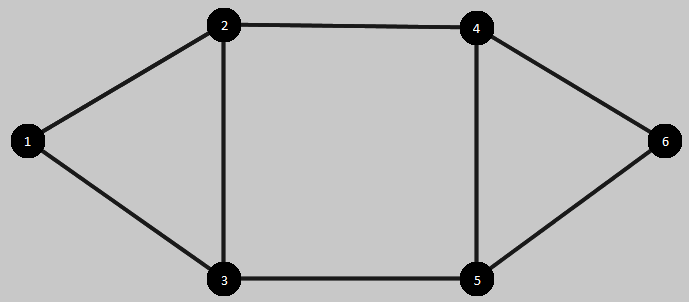
\includegraphics[width=13cm]{sdf/heuristic/figures/topological_design1}
\caption{Allowed physical topology of the reference network.}
\label{allowed_physical_surv_ref_low_heuristic}
\end{figure}

Following all the steps mentioned in the \ref{net2plan_guide}, applying the routing and grooming heuristic algorithms in the Net2Plan software and using all the data referring to this scenario, the obtained result can be consulted in the following table:

\begin{table}[H]
\centering
\begin{tabular}{|| c | c | c | c | c | c | c ||}
 \hline
 \multicolumn{7}{|| c ||}{CAPEX of the Network} \\
 \hline
 \hline
 \multicolumn{3}{|| c |}{ } & Quantity & Unit Price & Cost & Total \\
 \hline
 \multirow{3}{*}{Link Cost} & \multicolumn{2}{ c |}{OLTs} & 16 & 15 000 \euro & 240 000 \euro & \multirow{3}{*}{250 520 000 \euro} \\ \cline{2-6}
 & \multicolumn{2}{ c |}{100 Gb/s Transceivers} & 500 & 5 000 \euro/Gb/s & 250 000 000 \euro & \\ \cline{2-6}
 & \multicolumn{2}{ c |}{Amplifiers} & 70 & 4 000 \euro & 280 000 \euro & \\
 \hline
 \multirow{9}{*}{Node Cost} & \multirow{7}{*}{Electrical} & EXCs & 6 & 10 000 \euro & 60 000 \euro & \multirow{9}{*}{50 062 590 \euro} \\ \cline{3-6}
 & & ODU0 Ports & 60 & 8 \euro/Gb/s & 600 \euro & \\ \cline{3-6}
 & & ODU1 Ports & 50 & 6 \euro/Gb/s & 750 \euro & \\ \cline{3-6}
 & & ODU2 Ports & 16 & 3 \euro/Gb/s & 480 \euro & \\ \cline{3-6}
 & & ODU3 Ports & 6 & 1.5 \euro/Gb/s & 360 \euro & \\ \cline{3-6}
 & & ODU4 Ports & 4 & 1 \euro/Gb/s & 400 \euro & \\ \cline{3-6}
 & & Line Ports & 500 & 1 000 \euro/Gb/s & 50 000 000 \euro & \\ \cline{2-6}
 & \multirow{2}{*}{Optical} & OXCs & 0 & 20 000 \euro & 0 \euro & \\ \cline{3-6}
 & & Ports & 0 & 2 500 \euro/porto & 0 \euro & \\
 \hline
 \multicolumn{6}{|| c |}{Total Network Cost} & 300 582 590 \euro \\
\hline
\end{tabular}
\caption{Table with detailed description of CAPEX}
\label{scriptopaque_protec_ref_medium_heuristic}
\end{table}

Through the formulas mentioned below it can be demonstrated how all the values of the quantity column were calculated.

\begin{equation*}
 OLTs: 2 \sum_{(i,j):i<j}L_{ij} \qquad \qquad
 Transceivers: 2 \sum_{(i,j):i<j}W_{ij} \qquad \qquad
 Amplifiers: \sum_{(i,j):i<j}N^R_{ij} L_{ij} \\
\end{equation*}
\begin{equation*}
 EXCs: \sum_n^N N_{EXC,n} \qquad
 ODU0: \sum_{(o,d)}^{N}D_{od,0} \qquad \qquad
 ODU1: \sum_{(o,d)}^{N}D_{od,1} \qquad
 ODU2: \sum_{(o,d)}^{N}D_{od,2}
\end{equation*}
\begin{equation*}
 ODU3: \sum_{(o,d)}^{N}D_{od,3} \qquad \qquad
 ODU4: \sum_{(o,d)}^{N}D_{od,4} \qquad \qquad
 Line: \sum_{(i,j)}^{N}W_{ij}
\end{equation*}

\vspace{13pt}
$OXCs: \sum_n^N N_{OXC,n}$ but as mentioned initially this result is always zero \\

$Ports$: does not exist for this case then it is equal to zero \\

\textbf{High Traffic Scenario:}\\

In this scenario it has to take into account the traffic calculated in \ref{high_traffic_scenario}. In a first phase it will be shown the three topologies of the network, the first one already knew allowed physical topology, the second one allowed optical topology and finally the physical topology.\\

\textbf{10 Tbit/s}

\begin{figure}[H]
\centering
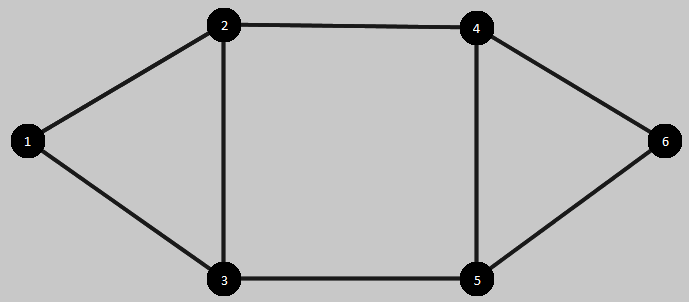
\includegraphics[width=13cm]{sdf/heuristic/figures/topological_design1}
\caption{Allowed physical topology of the reference network.}
\label{allowed_physical_surv_ref_low_heuristic}
\end{figure}

Following all the steps mentioned in the \ref{net2plan_guide}, applying the routing and grooming heuristic algorithms in the Net2Plan software and using all the data referring to this scenario, the obtained result can be consulted in the following table:

\begin{table}[H]
\centering
\begin{tabular}{|| c | c | c | c | c | c | c ||}
 \hline
 \multicolumn{7}{|| c ||}{CAPEX of the Network} \\
 \hline
 \hline
 \multicolumn{3}{|| c |}{ } & Quantity & Unit Price & Cost & Total \\
 \hline
 \multirow{3}{*}{Link Cost} & \multicolumn{2}{ c |}{OLTs} & 16 & 15 000 \euro & 240 000 \euro & \multirow{3}{*}{497 520 000 \euro} \\ \cline{2-6}
 & \multicolumn{2}{ c |}{100 Gb/s Transceivers} & 994 & 5 000 \euro/Gb/s & 497 000 000 \euro & \\ \cline{2-6}
 & \multicolumn{2}{ c |}{Amplifiers} & 70 & 4 000 \euro & 280 000 \euro & \\
 \hline
 \multirow{9}{*}{Node Cost} & \multirow{7}{*}{Electrical} & EXCs & 6 & 10 000 \euro & 60 000 \euro & \multirow{9}{*}{99 462 590 \euro} \\ \cline{3-6}
 & & ODU0 Ports & 60 & 8 \euro/Gb/s & 600 \euro & \\ \cline{3-6}
 & & ODU1 Ports & 50 & 6 \euro/Gb/s & 750 \euro & \\ \cline{3-6}
 & & ODU2 Ports & 16 & 3 \euro/Gb/s & 480 \euro & \\ \cline{3-6}
 & & ODU3 Ports & 6 & 1.5 \euro/Gb/s & 360 \euro & \\ \cline{3-6}
 & & ODU4 Ports & 4 & 1 \euro/Gb/s & 400 \euro & \\ \cline{3-6}
 & & Line Ports & 994 & 1 000 \euro/Gb/s & 99 400 000 \euro & \\ \cline{2-6}
 & \multirow{2}{*}{Optical} & OXCs & 0 & 20 000 \euro & 0 \euro & \\ \cline{3-6}
 & & Ports & 0 & 2 500 \euro/porto & 0 \euro & \\
 \hline
 \multicolumn{6}{|| c |}{Total Network Cost} & 596 982 590 \euro \\
\hline
\end{tabular}
\caption{Table with detailed description of CAPEX}
\label{scriptopaque_protec_ref_high_heuristic}
\end{table}

Through the formulas mentioned below it can be demonstrated how all the values of the quantity column were calculated.

\begin{equation*}
 OLTs: 2 \sum_{(i,j):i<j}L_{ij} \qquad \qquad
 Transceivers: 2 \sum_{(i,j):i<j}W_{ij} \qquad \qquad
 Amplifiers: \sum_{(i,j):i<j}N^R_{ij} L_{ij} \\
\end{equation*}
\begin{equation*}
 EXCs: \sum_n^N N_{EXC,n} \qquad
 ODU0: \sum_{(o,d)}^{N}D_{od,0} \qquad \qquad
 ODU1: \sum_{(o,d)}^{N}D_{od,1} \qquad
 ODU2: \sum_{(o,d)}^{N}D_{od,2}
\end{equation*}
\begin{equation*}
 ODU3: \sum_{(o,d)}^{N}D_{od,3} \qquad \qquad
 ODU4: \sum_{(o,d)}^{N}D_{od,4} \qquad \qquad
 Line: \sum_{(i,j)}^{N}W_{ij}
\end{equation*}

\vspace{13pt}
$OXCs: \sum_n^N N_{OXC,n}$ but as mentioned initially this result is always zero \\

$Ports$: does not exist for this case then it is equal to zero \\

\clearpage

\subsection{Transparent without Survivability}\label{heuristic_Transp_Survivability}
\begin{tcolorbox}	
\begin{tabular}{p{2.75cm} p{0.2cm} p{10.5cm}} 	
\textbf{Student Name}  &:& Pedro Coelho    (March 01, 2018 - )\\
\textbf{Goal}          &:& Implement the heuristic model for the transparent transport mode without survivability.
\end{tabular}
\end{tcolorbox}

\subsubsection{Model description}

\subsubsection{Result description}

\clearpage

\subsection{Transparent with 1+1 Protection}\label{heuristic_Transp_Protection}
\begin{tcolorbox}	
\begin{tabular}{p{2.75cm} p{0.2cm} p{10.5cm}} 	
\textbf{Student Name}  &:& Pedro Coelho    (March 01, 2018 - )\\
\textbf{Goal}          &:& Implement the heuristic model for the transparent transport mode with 1 plus 1 protection.
\end{tabular}
\end{tcolorbox}

\subsubsection{Model description}

\subsubsection{Result description}


\clearpage

\subsection{Translucent without Survivability}\label{heuristic_Transluc_Survivability}
\begin{tcolorbox}	
\begin{tabular}{p{2.75cm} p{0.2cm} p{10.5cm}} 	
\textbf{Student Name}  &:& Pedro Coelho    (March 01, 2018 - )\\
\textbf{Goal}          &:& Implement the heuristic model for the translucent transport mode without survivability.
\end{tabular}
\end{tcolorbox}

\subsubsection{Model description}

\subsubsection{Result description} 
\clearpage

\subsection{Translucent with 1+1 Protection}\label{heuristic_Transluc_Protection}
\begin{tcolorbox}	
\begin{tabular}{p{2.75cm} p{0.2cm} p{10.5cm}} 	
\textbf{Student Name}  &:& Pedro Coelho    (March 01, 2018 - )\\
\textbf{Goal}          &:& Implement the heuristic model for the translucent transport mode with 1 plus 1 protection.
\end{tabular}
\end{tcolorbox}

\subsubsection{Model description}

\subsubsection{Result description} 
%Section OPEX
%Subsection with the different transport mode 